\documentclass[12pt]{article}

\usepackage{sbc-template}


\usepackage{graphicx}
\usepackage{pythontex} 
\usepackage[brazil]{babel}   
\usepackage[utf8]{inputenc}  
\usepackage{circuitikz}


\sloppy

\title{Análise do Circuito RC}

\author{Pedro Henrique Gomes\inst{1}, Sarah Pereira Cerqueira\inst{2} }


\address{Departamento de Tecnologia (DTEC) -- Universidade Estadual de Feira de Santana
  (UEFS)\\
  Caixa Postal 252 e 294 -- 44036-900 -- Feira de Santana -- BA -- Brazil
  \email{ peuh\_fsa@hotmail.com,
  sarahecomp@gmail.com}
}

\begin{document} 

\maketitle
\begin{abstract}

\end{abstract}

\begin{resumo}
O presente documento faz uma análise do circuito RC em série  no domínio da frequência
\end{resumo}

 \section{Introdução}
 O circuito resistor-capacito (RC), é um dos filtros eletrônicos mais simples e básico da eletrônica. Ele consiste em um capacitor e um resistor ligados em série ou paralelo, alimentados por uma fonte de tensão. 
 Diferente de circuitos puramente resistivos, cuja aplicação das leis de Kirchhoff resulta numa equação algébrica, a aplicação das leis de Kirchhorff em um circuito RC produz uma equação diferencial, que é mais difícil  de resolver. 
 
 \section Metodologia

\section{Diagrama do Circuito}

%DESENHO DO CIRCUITO
\begin{center}
\begin{circuitikz}[scale=1.6, transform shape][american voltages]
\draw 
(0,0){to[american voltage source, invert, l=$Vi$, color=red] (0,2) }
 to[R, l=$R$, i=$i$] (2,2)
 to[capacitor, v^>=$Vo$] (2,0) -- (0,0)
 ;\end{circuitikz}
 \end{center}

 %ANÁLISE DO CIRCUITO

 
 \section{Análise do Circuito}
A reatância e a Indutância num capacitor podem ser descritas por:

\begin{equation}
Xc = \frac{1}{w.C}\\
\end{equation}

\begin{equation}
Zc = Xc.j\\
\end{equation}

logo:

\begin{equation}
Zc = \frac{j}{w.C}\\
\end{equation}

Aplicando o divisor de Tensão:

\begin{equation}
Vo(w)=\frac{Zc.Vi}{Zc+Zr}
\end{equation}

Sabemos que a impedância Zr no resistor vale:

\begin{equation}
Zr= R
\end{equation}


Agora substituindo (3) em (4), 

\begin{equation}
Vo(w)=\frac{\frac{j.Vi}{w.C}}{\frac{j}{w.C} + R}
\end{equation}

Simplificando esse resultado, temos: 

\begin{equation}
Vo(w)=\frac{1.Vi}{1+jwRC}
\end{equation}

Portanto, a resposta em frequência desse circuito é expressa por:
\begin{equation}
\frac{Vo(w)}{Vi(w)}=\frac{1}{1+jwRC}
\end{equation}

Como solicitado, consideraremos R.C = 1, então temos:

\begin{equation}
\frac{Vo(w)}{Vi(w)}=\frac{1}{1+j.w}
\end{equation}

Por fim, fazendo \textit{s} = j.w o resultado final será:

\begin{equation}
\frac{Vo(s)}{Vi(s)}=\frac{1}{1+\textit{s}}
\end{equation}

\section{Resultados}
O gráfico da Figura 1 exibe o comportamento da equação (10), onde o eixo das abicissas é variável independente  \textit{s}. 

\begin{figure}[h]
\centering
\begin{pycode}

from pyx import *

g = graph.graphxy(width=8)
g.plot(graph.data.function("y(x)=1/(x+1)", min=0, max=50))
g.writePDFfile("function")
print (r'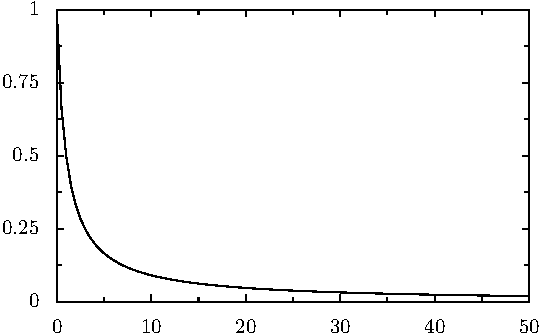
\includegraphics{function}')
\end{pycode}
\caption{$\frac{Vo(s)}{Vi(s)}=$$\frac{1}{1+s}$}
\end{figure}

\section{Referências}


\bibliographystyle{sbc}
\bibliography{sbc-template}

\end{document}
